The aim of hadron spectroscopy is to understand the observed experimental spectrum of hadrons in terms of the underlying theory of quarks and gluons, QCD. Traditionally, attempts to decipher the regularities present in the hadron spectrum have focussed on models having only limited connection to QCD; lattice QCD, which offers a first-principles approach to the theory, has now matured to the point where it is vital to efforts to understand excited hadrons.

In broad terms, one aim of the field is to discover how QCD arranges to have such regularity in the excited spectrum of hadrons, where the bulk of observed meson states can be understood as excitations of a $q\bar{q}$ system and baryons as $qqq$, and to understand whether or not there are states dominated by configurations of higher numbers of quarks (tetraquarks, pentaquarks), or configurations featuring only glue (glueballs), or excited glue coupled to quarks (hybrids). These latter possibilities, most of which are not yet unambiguously observed in experiments, come with potential smoking gun signatures of exotic flavor and/or $J^{PC}$ quantum numbers not accessible to a simple $q\bar{q}$ system~\cite{Meyer:2015eta} ($J$, $P$, $C$ refer to the total angular momentum, parity and charge conjugation properties respectively). Within the established hadron spectrum there are states which pose longstanding mysteries such as the light scalar mesons, $a_0(980), f_0(980)$, where diverse model-dependent explanations have been proposed that include tetraquark configurations and meson-meson molecular structure. Ultimately, an understanding of such states must come from QCD.

Our understanding of the excited hadron spectrum continues to be refined through data obtained in contemporary experimental programs (such as COMPASS, GlueX, CLAS12, BES III, LHCb) which are collecting unprecedented statistics with both established and novel production mechanisms. Observations made by these experiments are introducing new mysteries, such as the ``XYZ'' states in the charmonium region which do not fit into the previously successful modelling of charmonium~\cite{Lebed:2016hpi,Guo:2017jvc}. Near future experiments like Belle II and PANDA promise continued new information in particular in the bottomonium and charmonium sectors, and LQCD studies of the relevant spectra will continue to play a vital role in the interpretation of the experimental results in the context of QCD.


%%%%%%%%%%%%%%%%%%%%%%%%%%%%%%%%%%%%%%%%%%%%%%%%%%%%%%%%%%%%%%%%%%%%%%%%%%%%%%%%%%%%%%%%%%%%%%%%%%%%%%%%%%%%%%%%%%%
\subsection{Light hadron spectroscopy}

The lightest hadrons such as the neutron, proton, pion and kaon are stable against decay within QCD, and their mass and other properties can be computed with precision within lattice QCD by controlling the systematic uncertainties introduced through the lattice spacing, lattice volume and choice of quark mass. When the effects of electromagnetism are additionally accounted for, excellent agreement is found between theory and experiment~\cite{Duncan:1996xy,Blum:2007cy,Borsanyi:2014jba,Horsley:2015eaa,Blum:2010ym,Aoki:2012st,deDivitiis:2013xla}.

Unlike these lightest few states, the vast majority of the hadrons which appear in the Particle Data Tables~\cite{Patrignani:2016xqp} are \emph{unstable resonances}, which decay rapidly to lighter hadrons, and whose existence is inferred from enhancements in multi-hadron final states. Decades of accumulated data has led to an experimental spectrum in which each state may be broadly characterized in terms of a mass, a decay width, and branching fractions describing how often the state ends up in each possible decay mode. 

Earlier LQCD calculations considered the excited hadron spectrum in a simplified manner -- in the case of mesons, a large basis of fermion bilinear operators was used to construct a matrix of correlation functions, which was diagonalized to yield a discrete spectrum of excited state energies. The resulting spectra, determined for isospin, $I=1$, $I=0$ and charmonium~\cite{Dudek:2010wm,Dudek:2013yja, Liu:2012ze} show many of the regularities present in the experimental meson spectrum, but in addition show something not yet unambiguously observed, a clear spectrum of \emph{hybrid mesons}, some with exotic values of $J^{PC}$. Corresponding calculations of the baryon spectrum \cite{Dudek:2012ag} show the presence of a spectrum of \emph{hybrid baryons}, and a phenomenology has been built to describe these observations in QCD \cite{Dudek:2011bn}. 

While these calculations, performed at heavier than physical quark masses, give us a tantalizing glimpse of what lattice QCD can tell us about the hadron spectrum, they are not complete in that the hadronic decay physics of the states is not present in any controlled way -- the excited states are appearing as though they were stable states of definite mass rather than as resonances, and the spectrum obtained is at best a guide to the presence of relatively narrow resonances in a given energy region.

\begin{figure*}
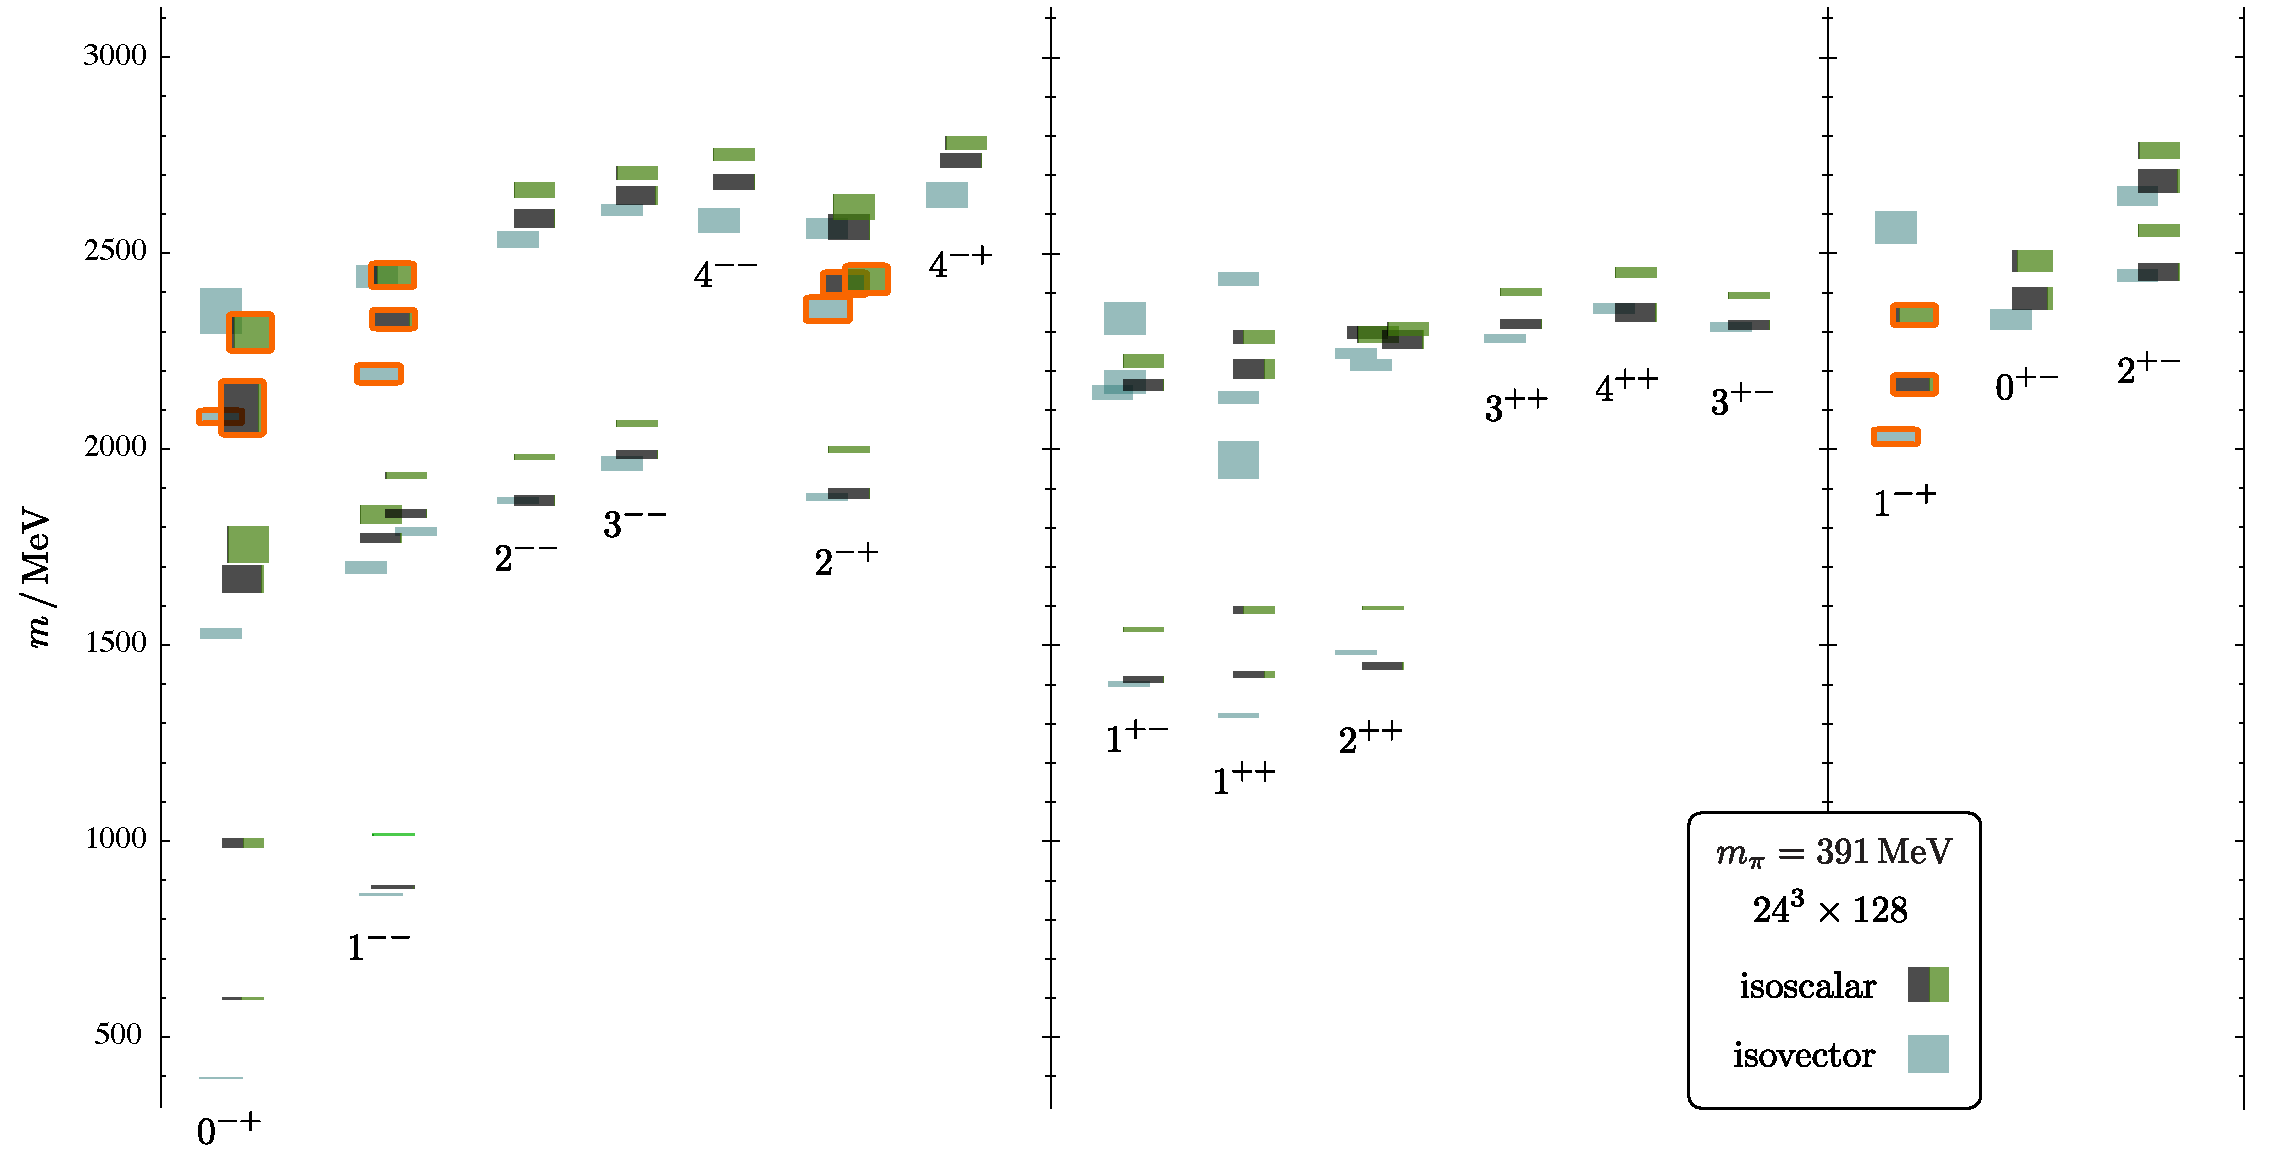
\includegraphics[width=0.88\textwidth]{figures/isoscalar}
\caption{The spectrum of excited mesons of various $J^{PC}$ extracted from a lattice QCD calculation with light quark masses such that $m_\pi = 391$ MeV \cite{Dudek:2013yja}. The lightest set of states identified as \emph{hybrid mesons} appear with an orange outline.}
\label{spectrum}
\end{figure*}

In order for a QCD calculation to be a faithful reflection the relevant physics, it must be capable of resolving excited hadrons as they truly are, as short-lived resonances, typically decaying to more than one final-state. This necessitates the computation of the energy-dependence of coupled-channel scattering amplitudes, in which the resonances will appear as enhancements. In the past five years, USQCD collaboration members have made significant progress in determining such amplitudes, making use of relations which connect them to the discrete spectrum of eigenstates of quantum field theory in a finite-volume, which can be computed in LQCD
\cite{Luscher:1986pf,Luscher:1990ux,Rummukainen:1995vs,Feng:2004ua,He:2005ey,Bedaque:2004kc,Liu:2005kr,Kim:2005gf,Christ:2005gi,Lage:2009zv,Bernard:2010fp,Fu:2011xz,Gockeler:2012yj,Leskovec:2012gb,Briceno:2012yi,Hansen:2012tf,Guo:2012hv,Li:2012bi,Briceno:2013hya,Briceno:2014oea}.

The simplest case is elastic scattering, where in a limited energy region only one hadron-hadron channel is kinematically open. Resonances appearing in elastic scattering include the $\rho$ and the $\sigma$ in $\pi\pi$ scattering, the $K^\star$ in $\pi K$, and the $\Delta$ in $\pi N$, all of which have been considered in LQCD~\cite{Aoki:2007rd,Feng:2010es,Lang:2011mn,Aoki:2011yj,Dudek:2012xn,Pelissier:2012pi,Wilson:2015dqa,Bali:2015gji,Bulava:2016mks,Guo:2016zos,Briceno:2016mjc,Guo:2018zss,Bali:2015gji,Lang:2012sv,Fu:2012tj,Prelovsek:2013ela,Brett:2018jqw,Andersen:2017una}.
%
In the elastic case, the scattering amplitude can be described by a single real energy-dependent parameter, the phase-shift, which has a characteristic rise through $90^\circ$ if a narrow resonance is present. For elastic scattering, there is a simple one-to-one mapping of each discrete energy level in a finite-volume to a value of the elastic scattering phase-shift at that energy (neglecting higher partial waves) \cite{Luscher:1986pf,Luscher:1990ck}. It follows that the lattice calculation is required to have a robust determination of the discrete spectrum of eigenstates, ideally in several lattice volumes. Additionally, the use of moving frames \cite{Rummukainen:1995vs} and/or asymmetrical volumes \cite{Li:2003jn,Detmold:2004qn}, can give access to more energy values which can be used to map out the energy dependence of the phase-shift. To more reliably extract the complete spectrum of eigenstates it proves necessary to go beyond the kind of ``single-hadron-like'' operator basis used in the simplified  spectrum calculations described above, and to also include a set of operators which resemble the relevant hadron-hadron pair undergoing the scattering process.

The LQCD technology of operator and correlation function construction has been developed to a state where these elastic scattering calculations are becoming a standard component of the USQCD program and are being pursued by groups around the world \cite{Aoki:2007rd,Feng:2010es,Lang:2011mn,Aoki:2011yj,Dudek:2012xn,Pelissier:2012pi,Mohler:2012na,Prelovsek:2013cra,Lang:2014yfa,Bali:2015gji,Lang:2015sba,Lang:2016jpk,Bulava:2016mks}. Recent examples are presented in Fig~\ref{elastic} for the case of $\pi\pi$ scattering in $I=1$ and $I=0$, where the very different behavior of the $\rho$ resonance and the $\sigma$ can be observed. LQCD~\cite{Briceno:2016mjc} has shown for the first time in a first-principles approach to QCD, that the $\sigma$ meson evolves from being a broad resonance at light quark masses~\cite{Guo:2018zss}, into a stable bound-state below the $\pi\pi$ threshold. 

\begin{figure}
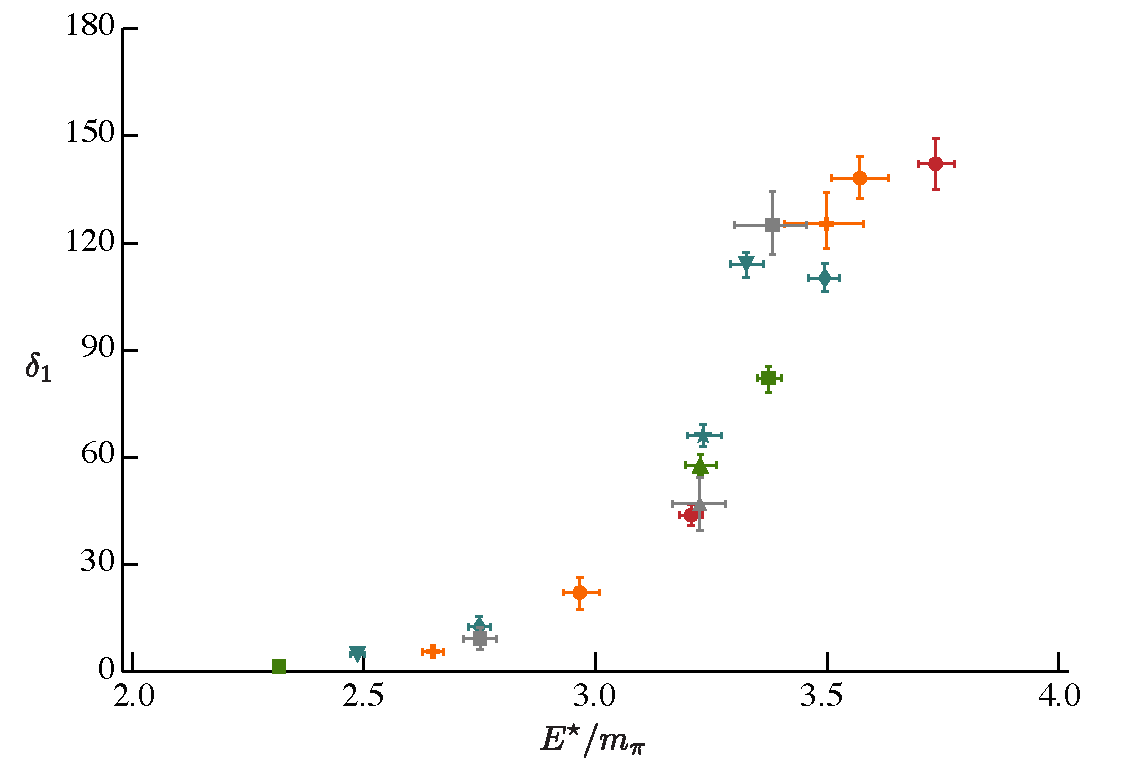
\includegraphics[width=0.44\textwidth]{figures/bulava}
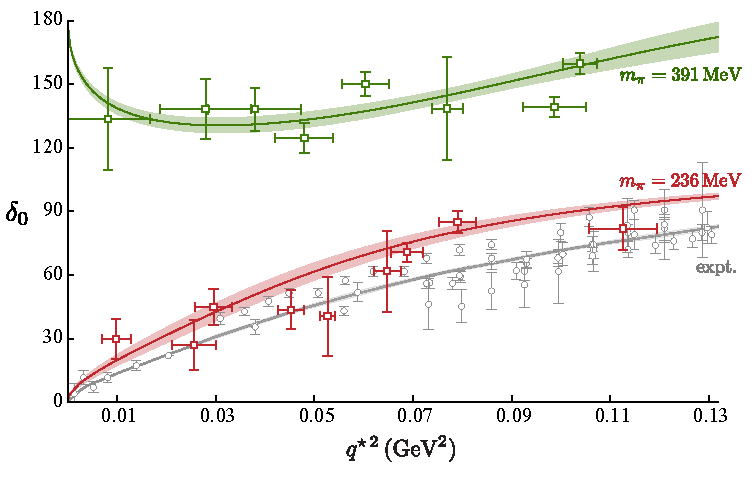
\includegraphics[width=0.48\textwidth]{figures/sigma}
\caption{$\pi\pi$ elastic scattering phase-shifts from lattice QCD calculations. (a) Isospin=1 $P$-wave computed with $m_\pi \sim 236$ MeV~\cite{Bulava:2016mks} showing the characteristic narrow $\rho$ resonance. (b) Isospin=0 $S$-wave at $m_\pi \sim 391$ MeV and $m_\pi \sim 236$ MeV where the $\sigma$ meson appears as a bound-state, broad resonance respectively~\cite{Briceno:2016mjc}.}
\label{elastic}
\end{figure}


Going beyond the simplest case of elastic scattering, resonances will appear in the \emph{coupled-channel $S$-matrix}. When more than one hadron-hadron channel is open, the lattice spectrum calculations require extension of the operator basis to include hadron-hadron operators of the relevant species, but the analysis to turn this spectrum into information about scattering is less straightforward, since there can no longer be a one-to-one mapping of any given energy level into the multiple unknowns of a coupled-channel scattering matrix at that energy \cite{Luscher:1986pf}. A successful approach \cite{Dudek:2014qha,Wilson:2014cna,Wilson:2015dqa,Moir:2016srx,Dudek:2016cru,Briceno:2017qmb} has been to parameterize the energy-dependence of coupled-channel amplitudes, and to use very many discrete energy levels in multiple volumes and/or moving frames to constrain the free parameters. Potential bias introduced by explicit choice of parameterization can be reduced by considering a range of forms, and exploring to what extent the best-fit amplitudes vary with parameterization choice~\cite{Dudek:2014qha,Wilson:2014cna,Wilson:2015dqa,Moir:2016srx,Dudek:2016cru,Briceno:2017qmb}. Increasingly more sophisticated approaches such as unitarized chiral perturbation theory have also been considered~\cite{Doring:2011vk,Albaladejo:2016lbb}

Having explicit analytic forms for the amplitudes has the advantage that it becomes possible to determine resonance properties  by analytically continuing the parametrized amplitudes into the complex energy plane, with resonances appearing as pole singularities, and where the couplings of resonance states to their decay channels can be obtained from the pole residues. The real and imaginary parts of the pole position can be identified with the mass and total width of the resonance, and the couplings are related to the decay branching fractions.
%
This methodology was recently used to find low-lying scalar and tensor resonances in the coupled $\pi\pi, K\overline{K}, \eta\eta$ system with $I=0$. In Ref.~\cite{Briceno:2017qmb}, a calculation with quark masses corresponding to a pion mass $\sim$ 400 MeV was presented where excited state spectra were extracted from variational analysis of correlation matrices computed in three lattice volumes, in a range of moving frames. The resulting energies were used to constrain the various amplitudes shown in Fig.~\ref{f0f2}. The scalar amplitude has a highly non-trivial behavior in which a bound-state lying below $\pi\pi$ threshold interferes with an $f_0(980)$-like resonance singularity lying close to the $K\overline{K}$ threshold, leading to a {dip} in the $\pi\pi \to \pi \pi$ amplitude that is analogous to a feature seen in the experimental amplitude. The resonance is found to have roughly equal coupling strength to $\pi\pi$ and $K\overline{K}$. The tensor amplitude is quite different, being much closer to our expectations for straightforward resonant enhancements, with two clear peaks corresponding to two pole singularities, one coupled dominantly to $\pi\pi$ and the other to $K\overline{K}$; numerical estimates are determined for the branching fractions from the pole residues. These two resonances closely resemble the experimentally well established $f_2(1270), f_2'(1525)$ states.
%
This example illustrates the highly non-trivial dynamics that can arise in hadron-hadron scattering from the non-perturbative dynamics of QCD, and LQCD is for the first time providing us a methodology to explore this dynamics without recourse to approximations or assumptions whose justification may not be clear. 
%Lattice QCD is transitioning into being the tool of choice for the study of hadron spectroscopy.

%... also found a0(980) like state ... these scalar mesons long been a problem for simple pictures ... too much detail here ??

 
\begin{figure*}
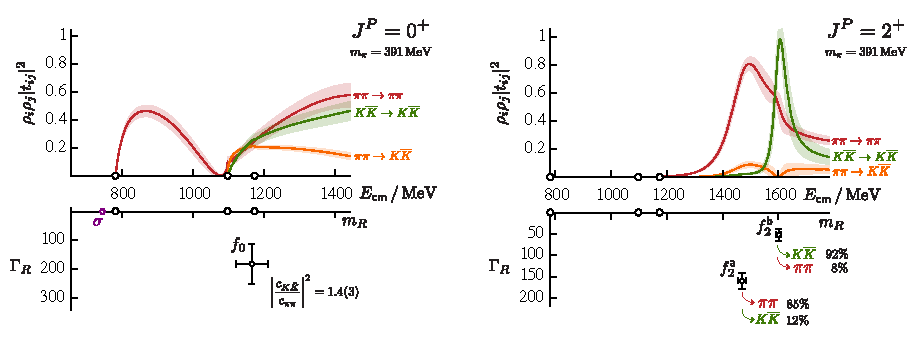
\includegraphics[width=0.95\textwidth]{figures/f0f2}
\caption{$\pi\pi, K\overline{K}$ coupled-channel scattering amplitudes in two partial-waves determined in a lattice QCD calculation with $m_\pi \sim 400$ MeV~\cite{Briceno:2017qmb}. (a) $J^P=0^+$ sector found to contain a bound-state $\sigma$, but also a resonance pole near the $K\overline{K}$ threshold, having strong coupling to both $K\overline{K}$ and $\pi\pi$ that may be associated with the experimental $f_0(980)$ meson. (b) $J^P=2^+$ sector found to contain two narrow tensor resonances.}
\label{f0f2}
\end{figure*}

A new generation of experiments are studying hadron spectroscopy using novel production mechanisms -- an example being the GlueX experiment at Jefferson Lab, which is producing meson resonances using a photon beam, with a particular focus being the search for exotic $J^{PC}$  mesons which may have an explanation as \emph{hybrids} featuring an excitation of the gluonic field. The anticipated huge data set from this experiment motivates study of the coupling of excited hadrons to photons, and in recent years we have seen the development of a formalism to extract the relevant amplitudes from finite-volume LQCD calculations \cite{Lellouch:2000pv,Lin:2001ek,Christ:2005gi,Hansen:2012tf,Briceno:2012yi,Bernard:2012bi,Agadjanov:2014kha,Briceno:2014uqa,Briceno:2015csa,Briceno:2015tza,Agadjanov:2016fbd}. Indeed, the first explicit calculation \cite{Briceno:2015dca,Briceno:2016kkp} computed three-point vector current correlation functions corresponding to the quantum numbers of the process $\gamma^\star \pi \to \pi \pi$ with $J^P=1^-$, in which the $\rho$ resonance is expected to appear. The results of this first calculation at $m_\pi \sim 400$ MeV are presented in Fig.~\ref{rhopigamma} where the effect of the $\rho$ resonance in the electromagnetic transition amplitude can be clearly observed, and where the dependence on the virtuality of current can be used to determine the \emph{transition form-factor} of the unstable $\rho$ resonance (see also \cite{Alexandrou:2018jbt}). The formalism for the analysis of  $e^+ e^-$ annihilation to meson-meson final-states through a photon has also been applied to $\rho \to \pi\pi$ decays~\cite{Feng:2014gba}.

Over the past ten years LQCD has transformed theoretical hadron spectroscopy, moving it from being dominated by model calculations, which while useful, had only a limited connection to QCD, to being directly connected with QCD with only controlled approximations made. Initial successes mapping out the highly excited spectrum of mesons and baryons, while excluding their decay properties, led to answers to longstanding questions about the role of excited gluonic fields in the hadron spectrum. More recently the field has begun computing excited hadrons as they truly are, as unstable resonances in hadron scattering amplitudes, firstly for the simple case of elastic resonances, and then for resonances which can decay into two or three different final states. The coupling of unstable resonances to external currents is now accessible in lattice QCD calculations, in some cases this provides an observable which can be compared to experiment, and in others a set of form-factors which can be used to build a space-time picture of the distribution of constituents within the unstable hadrons, potentially allowing for a validation of model-dependent claims that some states are e.g. diffuse meson-meson molecules. We are only beginning to see the possibilities of using lattice QCD to understand hadron spectroscopy, as has been highlighted in the 2015 NSAC Long Range Plan for Nuclear Science \cite{Geesaman:2015fha}.


\begin{figure}
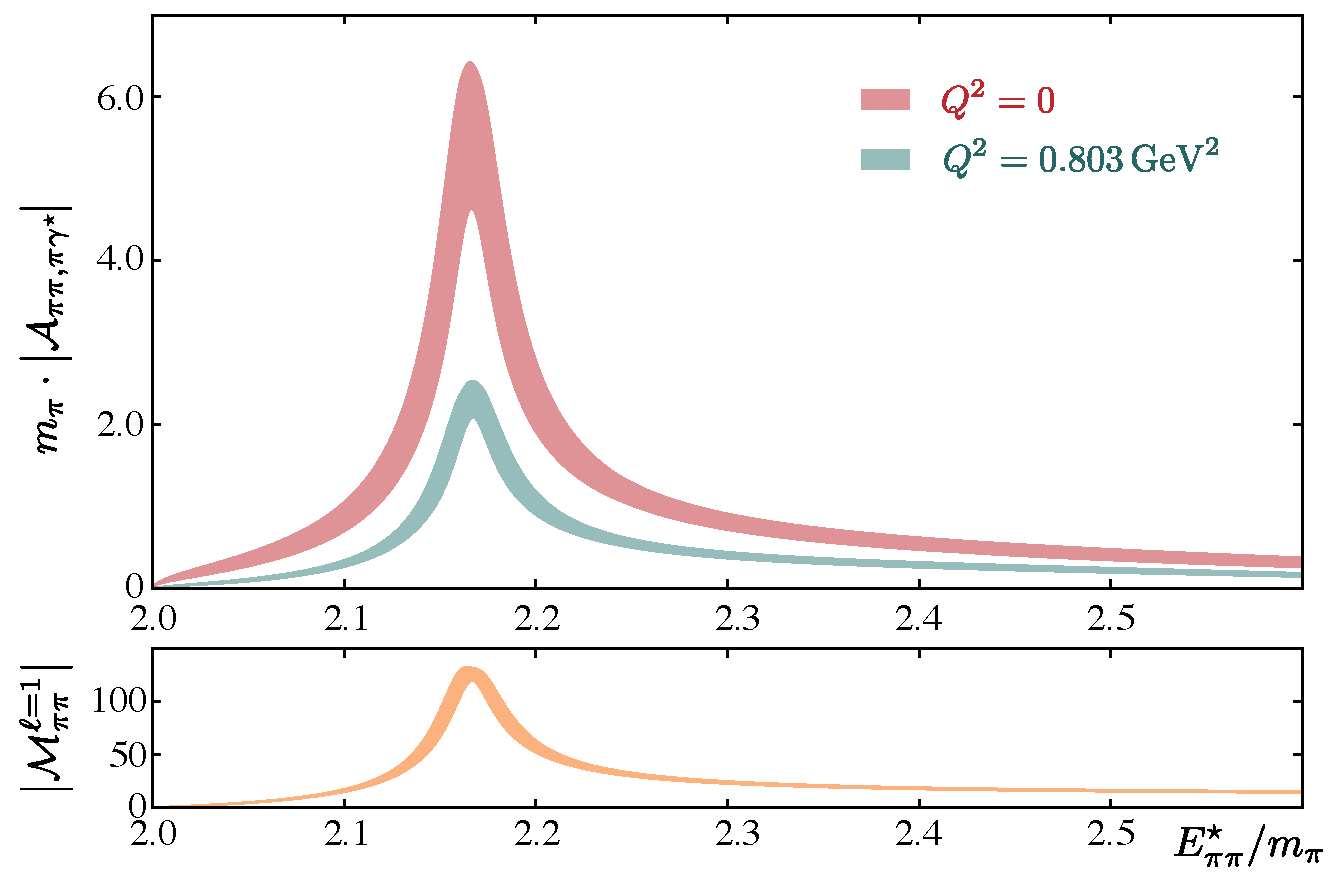
\includegraphics[width=0.95\columnwidth]{figures/rho_pi_gamma}
\caption{Amplitude for the process ${\pi \gamma^\star \to \pi\pi}$ in $P$-wave computed in lattice QCD with $m_\pi \sim 400$ MeV~\cite{Briceno:2016kkp,Briceno:2015dca}. Shown for two values of the photon virtuality, $Q^2$, and also shown the corresponding amplitude for $\pi\pi \to \pi \pi$ indicating that the $\rho$ resonance is contributing to both processes.  }
\label{rhopigamma}
\end{figure}

This physics progress comes about because of significant technical advances that have been made by USQCD in all aspects of LQCD calculations (see the  companion whitepaper of computational LQCD \cite{Joo:2019byq}). Operators have been developed which overlap efficiently with the eigenstates of QCD in a finite-volume, either as ``single-hadron'' operators or as constructions which resemble a pair of hadrons and which respect the cubic symmetry of the lattice. To compute the required correlation functions, diagrams featuring quark-antiquark ``annihilation'' lines are required, and techniques such as \emph{distillation}~\cite{Peardon:2009gh} and stochastic variants~\cite{Morningstar:2011ka} have rendered these, which were traditionally considered extremely challenging, now quite run-of-the-mill. The use of anisotropic lattices, in which the lattice spacing in the time direction is somewhat finer than in the spatial directions, has allowed for rather precise determinations of discrete energy spectra, through fine resolution of the time dependence of correlation functions. Anisotropic lattices have reduced the computational cost of such studies relative to working on fine isotropic lattices, particularly given the need to use relatively large volumes. The need to compute large matrices of correlation functions in order to accurately determine the discrete excited spectrum of QCD eigenstates, has had the consequence that the computation cost of the final stage of the lattice calculation, in which the correlation functions are constructed, has become a significant portion of the total computational budget. Much ongoing effort is devoted to identifying methods to reduce this cost. 


\paragraph{Future opportunities}

Looking forward, we expect to see much more progress in understanding the light hadron spectrum using lattice QCD methods. Early targets will see the application of established two-body techniques to channels that have not previously been explored. Proposed calculations include some to study the experimentally established axial meson resonances like $a_1$, $b_1$, which are known to have dominant decays to $\pi \rho$, $\pi \omega$. At heavier than physical light quark masses, the vector mesons in the decay are stable, and the decay is two-body. There are still novel challenges here associated with the additional spin degree-of-freedom provided by the vector: for example, the $J^{PC}=1^{+\pm}$ quantum numbers of the axial mesons can be constructed with either an $S$-wave or a $D$-wave between the pseudoscalar and the vector mesons. In a non-resonant case of $\pi \rho$ scattering with $I=2$ it has been shown that the relative strength of these two channels, and the mixing between them, can be determined in lattice QCD calculations~\cite{Woss:2018irj}. These techniques, once established for the axial meson resonances can be extended to other $J^{PC}$; an important case is the exotic $J^{PC}$ sector in which \emph{hybrid mesons} are predicted to appear. The larger mass of these resonances is such that several decay channels are kinematically accessible. The aim of the first calculations will be to predict some properties of these states in advance of the search within the GlueX data set, and in particular to have first estimates for the mass, total decay width, and the branching fractions to the various final states. This can be used to offer guidance to experiments like GlueX which have to select a particular set of final state particles for analysis when searching for resonances.

There are opportunities, as well as challenges, to understanding the low energy resonant spectrum of baryons. The first excitation of the proton -- the ``Roper'' -- is expected to be resonant in $N\pi$. At unphysical pion masses, the splitting of $N\pi$, $N\eta$ and $\Sigma K$ thresholds leaves only a small window to consider the resonance in an elastic region, thus it is expected that the use of the coupled channel formalism will be essential to adequately address this and other baryon systems. 

While the expectation is for calculations to progressively be done at lighter and eventually physical light quark masses, in the short-term, some calculations at heavier than physical quark masses will continue to be warranted. By increasing the light quark mass, pions become heavier, and three-meson thresholds correspondingly lie higher, providing a larger energy region over which the unique and well-studied two-body finite-volume formalism can be applied rigorously. 
At present, the absence of a complete formalism to describe three-hadron scattering in a finite-volume is an important  restriction. It is clear that this must be remedied if calculations are to proceed at lighter quark masses, where the bulk of resonances lie above at least one three-hadron threshold. On this front, a significant formal effort is underway \cite{Polejaeva:2012ut,Hansen:2015zga,Hansen:2014eka,Briceno:2018aml,Doring:2018xxx,Mai:2017bge,Mai:2018djl,Hammer:2017kms,Hammer:2017uqm} using a number of different approaches, and there is work ongoing to understand the commonalities in the results. On the practical lattice computational side, the extension of previous calculations is relatively straightforward -- three-hadron-like operators can be constructed using the same techniques used to combine single hadrons into two-hadron operators, and approaches like distillation \cite{Peardon:2009gh} allow for the relevant correlation functions to be computed without any additional computation of propagator objects. The increased number of quark fields involved will naturally lead to a combinatoric increase in contraction costs, and algorithmic improvements under the LQCD Exascale Computing Project and the LQCD SciDAC-4 project are being explored to reduce these costs.

While the development of a rigorous three-body (and higher) formalism is vital to have confidence in the calculations of high-lying resonances, it is likely that explicit calculations will show simpler behavior corresponding to quasi-two-body decays in many cases. Experimentally resonances appearing in three-body and higher multiplicity final state are observed to dominantly proceed through intermediate two-body states featuring isobar resonances which subsequently decay, e.g. $a_1 \to \rho \pi \to (\pi\pi) \pi$. It may eventually prove possible to make use of this isobar dominance to simplify somewhat the analysis of finite-volume spectra in energy regions in which three hadron and even higher multiplicity final states are kinematically accessible.

Building on the first successful calculations involving currents coupled to resonances, we will see extensions to other resonant states. Transition form-factors evaluated for photons with zero momentum transfer control the rate of photoproduction at GlueX -- first calculations (even for unphysically heavy quark masses) of established mesons can be compared to the first round of analysis of the GlueX data set, and prediction estimates made for the exotic $J^{PC}$ state production rates. Beyond electromagnetism, we will see calculations of light quark resonances appearing in weak heavy-flavor decays. This includes the flavor-changing neutral-current process $B \to \ell^+\ell^- \!\!\!\! \underset{\;\;\;\;\;\hookrightarrow K\pi}{K^*}$, in which there are currently tensions between theory and experiment that hint at physics beyond the Standard Model, and the charged-current decay $B \to \ell^-\bar{\nu}  \!\!\!\!\!\!\!\!\;\;\underset{\;\;\;\;\;\;\hookrightarrow \pi\pi}{\rho}$, which can provide new information on the $|V_{ub}|$ puzzle. More detailed discussions of these weak decays can be found in
the accompanying whitepaper on quark and lepton flavor physics \cite{Lehner:2019wvv}.

As described in Section~\ref{sec:hadronstructure}, there are opportunities to use the techniques developed for spectroscopic studies of resonances to investigate their three-dimensional gluon structure described by gluon GPDs and TMD. These quantities may provide insight from QCD into details of the nature of exotic states. These calculations are extremely demanding computationally and will also require continued theoretical development.






%%%%%%%%%%%%%%%%%%%%%%%%%%%%%%%%%%%%%%%%%%%%%%%%%%%%%%%%%%%%%%%%%%%%%%%%%%%%%%%%%%%%%%%%%%
\subsection{Heavy quarks and the XYZ states}

Since the  observation of the $X(3872)$ in 2003 \cite{Choi:2003ue}, an ever growing family of unexpected enhancements in the experimental studies of charmonium region have been seen, known colloquially as the ``XYZ'' states. These enhancements, if interpreted as resonances, typically lie outside the previously successful picture of charmonium in terms of $c\bar{c}$ bound-states, sometimes in extreme ways. For example the $Z_c$ enhancements observed in final states like $J/\psi \, \pi^+$ are \emph{charged}, and it is argued must have minimal quark content $c\bar{c} u \bar{d}$. Further discoveries and refined measurements of the properties of observed states continue in earnest at facilities like LHCb and BES III, with further extension into the bottomonium sector expected at Belle II.

Within the charm sector, the LQCD methods described above can be brought to bear on the question of flavor exotics and the other excess XYZ states. There have been suggestions that at least some of the observed experimental enhancements arise due to the kinematics of the three-body production process (e.g. $e^+e^- \to \pi \; (\pi J/\psi) $ or $B \to K \, (\psi' \pi)$), rather than being due to a true two-body resonance \cite{Guo:2015umn,Szczepaniak:2015eza}. Lattice calculations have the advantage here that in order to determine the resonant content, they are not restricted to studying particular higher-multiplicity production processes, but rather they can compute the two-body scattering amplitude directly, removing the effect of any kinematic singularities particular to the production mechanism.


The techniques for determination of coupled-channel scattering matrices pioneered in the light-quark sector and described in the previous section can be applied for heavy quarks. The calculations are somewhat more technically challenging as the small spin-splitting between $D$ and $D^*$ mesons, and the lightness of the $\pi$ compared to the energy gap between the $J/\psi$ and the relevant excited states, means that there are typically several kinematically accessible channels which must be considered.

The calculation of the radiative decay of the XYZ states can address the speculations of the `XYZ'-s are `molecular' in origin. First calculations could target the open-charm systems as well as the more challenging $I=0$ $D\bar{D}$ decays.
%
There are hints already that some of the experimentally observed enhancements may not have a resonant origin. In Ref.~\cite{Cheung:2017tnt} (see also \cite{Prelovsek:2014swa}), a lattice calculation of the spectrum of states with the quantum numbers of the $Z_c(3900)$, using a large basis of operators containing many resembling the expected finite-volume meson-meson states as well as several having tetraquark-like structure, showed no significant deviations from the spectrum expected if interactions are only weak, and no resonance is present. 

While the first LQCD studies suggest that double charm and hidden charm tetraquarks do not appear as entities in the spectrum, there is significant evidence from lattice calculations that double beauty tetraquarks are
actually {bound}~\cite{Francis:2016hui,Junnarkar:2018twb,Leskovec:2019ioa} (see also Refs.~\cite{Hughes:2017xie,Francis:2018jyb}). Such states, if they can be produced experimentally, would be observed through their weak decay. Further LQCD calculations, utilizing the diverse operator bases already shown to be capable of  reliably extracting the complete low-energy spectrum, are warranted to investigate systematics and determine the properties of these states with higher precision.

The spectrum and dynamics of hadrons containing heavy quarks are constrained by approximate heavy-quark flavor and spin symmetries
\cite{Korner:1994nh,Manohar:2000dt}. A particularly interesting symmetry emerges for doubly heavy baryons and doubly heavy tetraquarks: in the large-mass limit, the two heavy quarks
are expected to form a point-like diquark that acts like a single heavy antiquark, and the light degrees of freedom behave as in a
singly-heavy hadron \cite{Carlson:1987hh,Savage:1990di,Manohar:1992nd,Brambilla:2005yk,Eichten:2017ffp}. With the current operation of the LHC, charm and bottom baryons are being produced in unprecedented quantities.
This has led to several discoveries in the last few years \cite{Chatrchyan:2012ni,Aaij:2012da,Aaij:2014yka,Aaij:2016jnn,Aaij:2017ueg,Aaij:2017vbw,Aaij:2017nav,Aaij:2018yqz,Aaij:2018tnn}, with many more expected in the future. LQCD
can predict the masses, can help assign $J^P$ quantum numbers, and can also provide information on the structure and decay rates~\cite{Brown:2014ena,Padmanath:2015jea,Bali:2015lka,Can:2015exa,Alexandrou:2016xok,Bahtiyar:2018vub,Woloshyn:2016pid,Alexandrou:2017xwd,Mathur:2018epb,Mathur:2018rwu}. Including the effects of electromagnetism and isospin breaking even allows estimates of charge splittings for stable states~\cite{Borsanyi:2014jba}.

The LHCb collaboration has reported the observation of three narrow $J/\psi\: p$ pentaquark resonances, $P_c(4312)$, $P_c(4440)$, and $P_c(4457)$, in $\Lambda_b \to J/\psi\,p\,K$ decays \cite{Aaij:2015tga,Aaij:2019vzc}.
Studying these resonances on the lattice is challenging due to the many open channels, including channels with more than two hadrons. Charmonium-nucleon
interactions have been investigated in lattice QCD at low energies \cite{Yokokawa:2006td,Liu:2008rza,Kawanai:2010ev,Beane:2014sda}, and recently also in the $P_c$ energy region \cite{Skerbis:2018lew}. The interactions near threshold were found to be slightly attractive, with an increasing attraction at unphysically heavy up and down quark quark masses, where bound states were seen \cite{Beane:2014sda}. The recent study of charmonium-nucleon interactions at higher energies \cite{Skerbis:2018lew} did not find any $P_c$ resonance, but the inclusion of additional channels (such as $\Sigma_c^+ \bar{D}^{0(*)}$) is expected to be important.




